%%%%%%
%
% $Author: Abishek $
% $Date: 06.05.2024 $
% $Path: BA24-02-Time-Series\report\Contents\en$
% $Version: 1.0 $
%
%
% !TeX encoding = utf8
% !TeX root = Rename
% !TeX TXS-program:bibliography = txs:///bibtex
\chapter{Documentation Developer}
\section{Structure}



The project is structured as follows:

\begin{verbatim}
	.
+-- models/
|   `-- gait_model.h           # Header file for Arduino integration
+-- src/
|   +-- dataloader.py          # Module to load CSV files
|   +-- kalmanfilter.py        # Kalman Filter for data smoothing
|   +-- cnnmodel.py            # CNN model creation and training
|   +-- visualization.py       # Visualization of predictions
|   +-- tfliteexporter.py      # Export to TensorFlow Lite and .h file
|   +-- config.py              # Configuration for pipeline parameters
|   +-- logger.py              # Logging setup
+-- data/
|   +-- normalpatterns.csv     # Gait data for normal patterns
|   `-- parkinsonpatterns.csv  # Gait data for Parkinson's patterns
`-- main.py                    # Entry point for the ML pipeline
README.txt                     # Project documentation
\end{verbatim}

\section{Idea}

The Parkinson Gait Pattern Recognition project aims to create a machine learning pipeline capable of differentiating between normal and Parkinsonian gait patterns. Using data collected from IMU sensors, the pipeline applies a Kalman Filter for data preprocessing and trains a CNN for binary classification. The trained model is exported in TensorFlow Lite format and integrated with Arduino Nano BLE Sense. Additionally, visualization tools are implemented to evaluate the model’s performance.

\section{Flowchart of Development Steps}
	\begin{figure}[h]
		
\centering
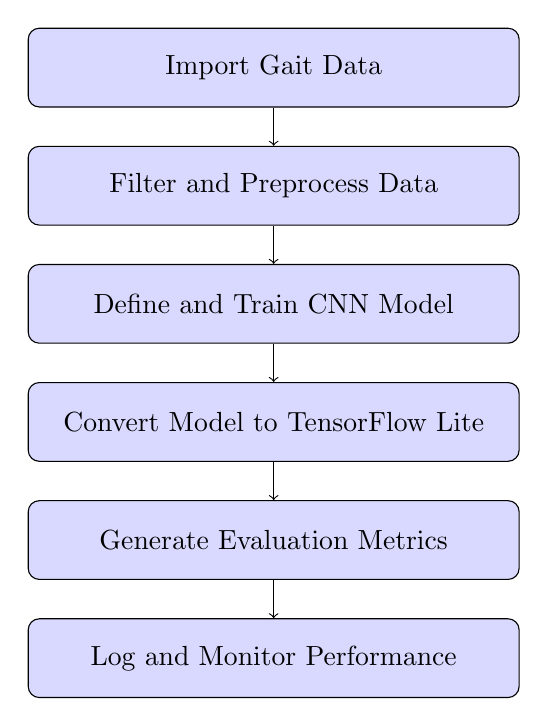
\begin{tikzpicture}[node distance=1.5cm, auto]
	% Define styles
	\tikzstyle{mainprocess} = [rectangle, draw, text width=6cm, align=center, fill=blue!15, rounded corners, minimum height=1cm]
	
	% Nodes
	\node[mainprocess] (data) {Import Gait Data};
	\node[mainprocess, below of=data] (preprocess) {Filter and Preprocess Data};
	\node[mainprocess, below of=preprocess] (train) {Define and Train CNN Model};
	\node[mainprocess, below of=train] (export) {Convert Model to TensorFlow Lite};
	\node[mainprocess, below of=export] (visualize) {Generate Evaluation Metrics};
	\node[mainprocess, below of=visualize] (logging) {Log and Monitor Performance};
	
	% Arrows
	\draw[->] (data) -- (preprocess);
	\draw[->] (preprocess) -- (train);
	\draw[->] (train) -- (export);
	\draw[->] (export) -- (visualize);
	\draw[->] (visualize) -- (logging);
\end{tikzpicture}
\caption{Flowchart of Development Steps}
\label{fig:Flowchart of Development Steps}
\end{figure}
\begin{enumerate}
	\item \textbf{Data Loading}:
	\begin{itemize}
		\item Load gait data from \texttt{normalpatterns.csv} and \texttt{parkinsonpatterns.csv}.
		\item Validate data consistency and completeness.
	\end{itemize}
	
	\item \textbf{Data Preprocessing}:
	\begin{itemize}
		\item Apply Kalman Filter to smooth noisy IMU data.
		\item Reshape data for CNN input.
	\end{itemize}
	
	\item \textbf{Model Training}:
	\begin{itemize}
		\item Create and train the CNN model on preprocessed data.
		\item Validate the model using a validation split.
	\end{itemize}
	
	\item \textbf{Model Export}:
	\begin{itemize}
		\item Convert the trained model to TensorFlow Lite format.
		\item Generate a \texttt{.h} file for Arduino integration.
	\end{itemize}
	
	\item \textbf{Visualization}:
	\begin{itemize}
		\item Use visualization tools to assess model predictions.
		\item Plot training accuracy and loss.
	\end{itemize}
	
	\item \textbf{Logging and Error Handling}:
	\begin{itemize}
		\item Log all major steps and errors during pipeline execution.
		\item Raise exceptions for critical failures.
	\end{itemize}
\end{enumerate}

\section{ML Pipeline}


\subsection{Steps in the ML Pipeline}

\begin{figure}[h]
	\centering
	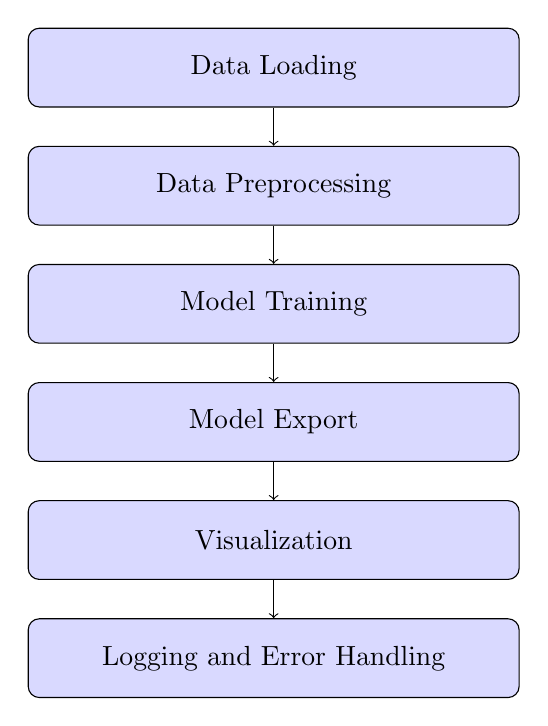
\begin{tikzpicture}[node distance=1.5cm, auto]
		% Define styles
		\tikzstyle{mainprocess} = [rectangle, draw, text width=6cm, align=center, fill=blue!15, rounded corners, minimum height=1cm]
		
		% Nodes
		\node[mainprocess] (data) {Data Loading};
		\node[mainprocess, below of=data] (preprocess) {Data Preprocessing};
		\node[mainprocess, below of=preprocess] (train) {Model Training};
		\node[mainprocess, below of=train] (export) {Model Export};
		\node[mainprocess, below of=export] (visualize) {Visualization};
		\node[mainprocess, below of=visualize] (logging) {Logging and Error Handling};
		
		% Arrows
		\draw[->] (data) -- (preprocess);
		\draw[->] (preprocess) -- (train);
		\draw[->] (train) -- (export);
		\draw[->] (export) -- (visualize);
		\draw[->] (visualize) -- (logging);
	\end{tikzpicture}
	\caption{Steps in the ML Pipeline}
	\label{fig:MLPipelineFlowchart}
\end{figure}




\begin{enumerate}
	\item \textbf{Data Loading}:
	\begin{itemize}
		\item The \texttt{dataloader.py} module reads CSV files containing gait data.
		\item Data is loaded into pandas DataFrames for processing.
	\end{itemize}
	
	\item \textbf{Data Preprocessing}:
	\begin{itemize}
		\item The \texttt{kalmanfilter.py} module smooths noisy data.
		\item Reshaped data is prepared for CNN input.
	\end{itemize}
	
	\item \textbf{Model Creation and Training}:
	\begin{itemize}
		\item The \texttt{cnnmodel.py} module defines CNN architecture and logs training progress.
	\end{itemize}
	
	\item \textbf{Model Export}:
	\begin{itemize}
		\item The \texttt{tfliteexporter.py} converts the model to TensorFlow Lite and generates \texttt{.h} file.
	\end{itemize}
	
	\item \textbf{Visualization}:
	\begin{itemize}
		\item The \texttt{visualization.py} provides tools to visualize training and test results.
	\end{itemize}
	
	\item \textbf{Logging and Configuration}:
	\begin{itemize}
		\item The \texttt{logger.py} manages logging.
		\item The \texttt{config.py} defines pipeline parameters.
	\end{itemize}
\end{enumerate}

\section{Example Usage}

\textbf{To execute the pipeline:}
\begin{enumerate}
	\item Install dependencies:
	\begin{verbatim}
		pip install -r requirements.txt
	\end{verbatim}
	
	\item Run the pipeline:
	\begin{verbatim}
		python main.py
	\end{verbatim}
\end{enumerate}

\section{Outputs}

\begin{itemize}
	\item \texttt{gait\_model.tflite}: TensorFlow Lite model for deployment.
	\item \texttt{models/gait\_model.h}: Header file for Arduino integration.
\end{itemize}

\section{Notes}

\begin{itemize}
	\item Ensure \texttt{normalpatterns.csv} and \texttt{parkinsonpatterns.csv} are present in the \texttt{data/} directory.
	\item Logs all major steps and handles exceptions to prevent pipeline interruptions.
\end{itemize}

This document provides a detailed guide to the Parkinson Gait Pattern Recognition project, ensuring developers understand each stage of the pipeline.

